\documentclass[12pt]{article}

%**********************************************
%* Add additional packages as needed

\usepackage{url,amsmath,setspace,amssymb}
\usepackage{listings}

\usepackage{tcolorbox}
\usepackage{tikz}
\usepackage{xcolor}


\usepackage{color}
\def\R{\color{red}}
\def\B{\color{blue}}

\usepackage{listings}
\usepackage{caption}


%**********************************************
%* Please replace this with your name and your AAU student number
\newcommand{\studentname}{Lorenzo Zanolin}
\newcommand{\studentnumber}{12245822}



%**********************************************
%* Some more or less useful stuff, add custom stuff as needed

\lstnewenvironment{myalgorithm}[1][] %defines the algorithm listing environment
{
   % \captionsetup{labelformat=algocaption,labelsep=colon}
    \lstset{ %this is the stype
        mathescape=true,
        frame=none,
        numbers=none,
        basicstyle=\normalsize,
        keywordstyle=\color{black}\bfseries\em,
        keywords={,input, output, return, datatype, function, in, if, else, foreach, while, begin, end, },
        numbers=left,
        xleftmargin=.04\textwidth,
        #1 % this is to add specific settings to an usage of this environment (for instance, the caption and referable label)
    }
}
{}


\newtcolorbox{alert}[1]{
colback=red!5!white, colframe=red!75!white,fonttitle=\bfseries, title = #1}

\newtcolorbox{commentbox}[1]{
colback=black!5!white, colframe=black!75!white,fonttitle=\bfseries, title = #1}



%**********************************************
%* Leave the page configuration as is
\setlength{\oddsidemargin}{.25in}
\setlength{\evensidemargin}{.25in}
\setlength{\textwidth}{6.25in}
\setlength{\topmargin}{-0.4in}
\setlength{\textheight}{8.5in}

\newcommand{\heading}[5]{
\renewcommand{\thepage}{#1-\arabic{page}}
\noindent
\begin{center}
	\framebox[\textwidth]{
	\begin{minipage}{0.9\textwidth} \onehalfspacing
	{\bf 622.755 -- \unitname} \hfill #2

	{\centering \Large #5

	}\medskip
	{#3 \hfill #4}
	\end{minipage}
}
\end{center}
}

\newcommand{\unitname}{Introduction to Cybersecurity}
\newcommand{\maxpages}{5}
\newcommand{\handout}[3]{\heading{#1}{#2}{\studentname}{\studentnumber}{#3}}
\bibliographystyle{plain}
%**********************************************
%* The document starts here
\begin{document}
\handout{\maxpages}{Summer Term, 2022/23}{Project Write Up}


\section{Outline}
Please write a general overview explaining the structure of your report. This can be brief (one paragraph), but it should make it clear how the report is structured. The overall length of your report must not exceed 5 pages (including figures, algorithms, tables, and references). This report is structured as follows: I will provide a brief overview of the the written project in Section \ref{sec:Overview}. Then I will explain how I would suggest you use your time to achieve a good write up in Section \ref{sec:Time}, and finally I will explain and illustrate the marking scheme in Section \ref{sec:Marking}.

\section{Yao's protocol}\label{sec:yao}
This project covers the Yao's protocol\cite{yao}; more precisely the \textit{Secure Multi-Party Computation}. This protocol allows two parties, Alice who knows x and Bob who knows y, to compute jointly the value of $f(x, y)$ in a way that does not reveal to each side more information than can be deduced from $f(x, y)$\cite{ot}.
In this scenario Alice is the garbler, while Bob is the evaluator. Another important role is the use of the \textit{OT}\cite{ot}, which is responsible to let Bob knows his encrypted input. An example of functioning is represented in figure \ref{steps}.

\begin{figure}[h]
    \makebox[\textwidth][c]{
    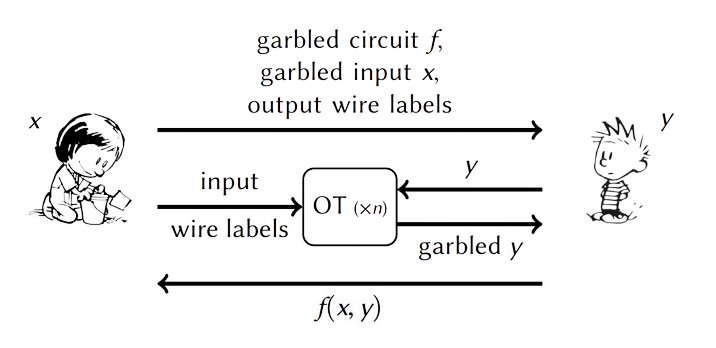
\includegraphics[width=1.1\linewidth]{../src/images/steps.png}}
    \caption{Steps of the SMPC}\label{steps}
\end{figure}

\footnote{\ref{steps} was taken from \url{https://web.engr.oregonstate.edu/~rosulekm/cryptabit/1-overview.pdf}
Image \ref{half} was taken from \url{https://upload.wikimedia.org/wikipedia/commons/1/14/Half-adder.svg}\\ 
Image \ref{full} was taken from \url{https://upload.wikimedia.org/wikipedia/commons/a/a9/Full-adder.svg}.}

There are two principles that must be respected\cite{principles}: 
\begin{itemize}
    \item \textit{privacy}: nothing is learned from the protocol other than the output;
    \item \textit{correctness}: the output is distributed according to the prescribed functionality.
\end{itemize}

The request was to implement a program for which two user can sum up their set of values without sharing them with the opposing party; in this case we decided to create a 8-bit adder circuit.
The circuit uses 7 full adders, 1 half adder and 1 if-then-else, represented in figures \ref{half} \ref{full} \ref{overflow}, concatenated together; the implementation of the entire circuit is represented in figure \ref{circuit}.

\begin{figure}[!htb]
    \begin{center}
        \begin{minipage}{0.4\textwidth}
            \centering
            
\includegraphics[width=.7\linewidth]{../src/images/Half_adder.png}
            \caption{Half Adder}\label{half}
        \end{minipage}
        \hfill
        \begin{minipage}{0.4\textwidth}
            \centering
            
\includegraphics[width=.8\linewidth]{../src/images/Full-adder.png}
            \caption{Full Adder}\label{full}
        \end{minipage}
        \hfill
        \begin{minipage}{0.45\textwidth}
            \centering
            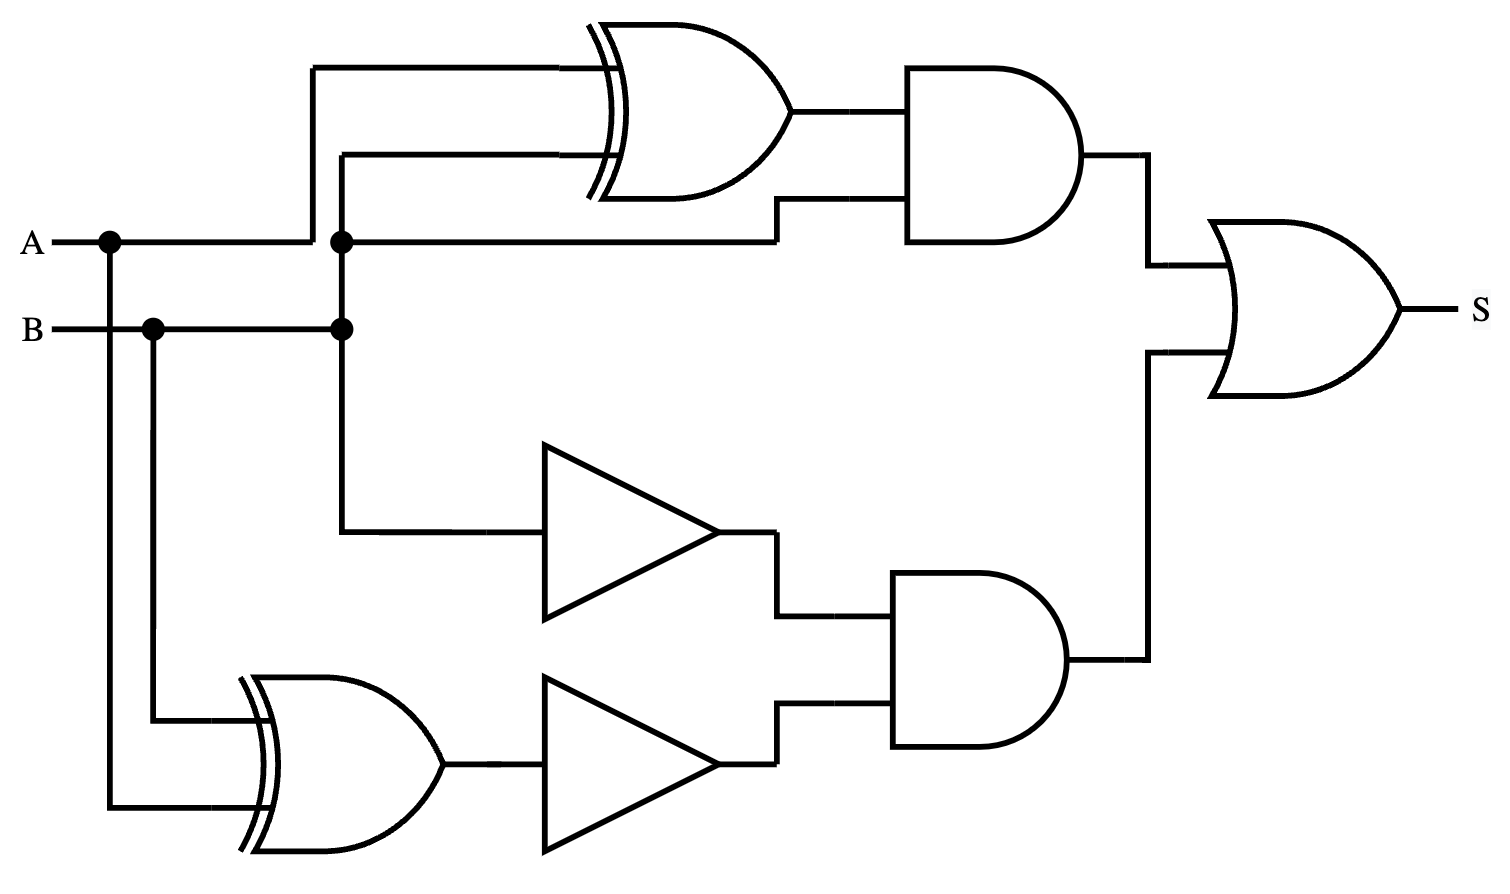
\includegraphics[width=1\linewidth]{../src/images/overflow.png}
            \caption{If then else}\label{overflow}
        \end{minipage}
    \end{center}
\end{figure}
\begin{figure}[!h]
    %\centering
    \makebox[\textwidth][c]{
    
\includegraphics[width=1.2\linewidth]{../src/images/Circuit.png}
    }
    \caption{8-bit Adder}\label{circuit}
\end{figure}



Full details of my implementation can be found at \url{https://github.com/lorenzozanolin/garbledCircuit}\label{zanoGit}.


\section{Real word application}\label{sec:world}
%manca esempio generico
\subsection{Average salary calculator}
In the \textit{sum} case, an example could be the following: imagine you are an employee in a corporation and you want to know the average salary without revealing to anyone your income. In this scenario you can the use the \textit{SMPC} protocol to get everyone's data and compute the sum; then you can proceede by calculating the mean. In this example anybody can understand values of other employees, thus \textit{privacy} is respected.
\section{Ethical, Legal and Social aspects}\label{sec:sel}

\section{Final considerations}

\bibliography{thud}
\end{document}



